% !TeX spellcheck = en_GB
% !TeX encoding = UTF-8

\documentclass{imeko_wc}
\usepackage[british]{babel}

\begin{document}

% ARTICLE TITLE
\title{Optical Profilometry Versus the Stylus: A Spectral Theory for Closing the Accuracy Gap}

% AUTHOR NAMES WITH AN AFFILIATION INDEX
\author[a1]{Dawid Kucharski}
\author[a1]{Micha{\l} Jakubowicz}

% AUTHOR AFFILIATIONS WITH THE CORRESPONDING INDEX
\affiliation[a1]{Institute of Mechanical Technology, Poznan University of Technology, Jacka Rychlewskiego 1 Street, 61-131 Pozna{\'n}, Poland}

% CORRESPONDING AUTHOR INDEX AND EMAIL
\CorrespondingAuthorNumber{1}
\CorrespondingAuthorEmail{dawid.kucharski@put.poznan.pl}

\maketitle % Print the title and abstract box

\begin{abstract}
Stylus profilometry and optical interferometry are compared in the spatial-frequency domain through a measurement-operator formalism computed from first-principles instrument physics. The stylus channel is modelled as morphological tip dilation with raster sampling; its empirical transfer is approximately flat with a curvature-bias excess, crossing \qty{3}{\decibel} only near the sampling scale. The optical channel follows the incoherent imaging transfer function with a diffraction cutoff of \qty{2000}{mm^{-1}}. A $k$-space equivalence regime covering \qty{9.6}{\percent} $\pm$ \qty{0.3}{\percent} of the measured bandwidth is identified at a crossover of \qty{454}{\per\milli\metre} $\pm$ \qty{165}{\per\milli\metre}. The optical model reproduces measured white-light-interferometry transfer functions from a public dataset, and all results are checked by eighteen automated verification tests. The study is computational and provides a falsifiable experimental roadmap.
\end{abstract}

\begin{keywords}
Surface metrology; instrument transfer function; stylus profilometry; white-light interferometry; power spectral density
\end{keywords}

\section{Introduction}

\label{sec:introduction}
Surface topography measurement supports quality control in precision manufacturing, functional design in tribology, and verification in optical fabrication. Two modalities dominate practice: contact stylus profilometry and non-contact optical interferometry, in particular white-light interferometry (WLI). Comparative studies date back three decades \cite{poon1995comparison}, and power spectral density (PSD) analysis has since become the standard for quantitative, scale-resolved surface characterisation \cite{jacobs2017quantitative}, in line with the paradigm shift towards information-rich surface metrology \cite{jiang2007paradigm}.

Most published comparisons, however, rely on scalar indicators such as the root-mean-square (rms) height error or the areal roughness \emph{Sa}. A single number of this kind cannot locate disagreement in scale: a stylus with a \qty{2}{\micro\metre} tip radius and an interferometer with NA 0.55 may return the same \emph{Sa} for one surface while disagreeing strongly on another. The spectral consequences of stylus-tip geometry have been analysed since the early simulations of Li and Devries \cite{li1984computer} and the tip-curvature spectral analyses of Wu \cite{wu1999spectral}; the instrument transfer function (ITF) of optical profilometers has been treated analytically by de Groot \cite{degroot2021itf} and measured experimentally with binary pseudo-random calibration artefacts \cite{yashchuk2015binary}. However, the two measurement principles have not been compared within one consistent $k$-space framework. Instrument bandwidth has been discussed qualitatively for surface measuring instruments \cite{leach2010bandwidth}, and the analytic PSD formalism and systematic spectral measurement errors have been catalogued in the lithography context \cite{mack2011analytic,mack2013systematic}; neither line of work, however, provides paired transfer functions for the tactile--optical comparison pursued here. The question left open is therefore scale-resolved: for a surface with a known PSD, what does each instrument in fact measure at each spatial frequency?

\section{Proposed Contribution}

\label{sec:contribution}
Every surface topography measurement is represented as a linear operator acting on the true height field $h(x,y)$, followed by additive noise:
\begin{equation}
\mathcal{M}[h(x,y)] = \mathcal{F}^{-1}\!\left[H(f_x,f_y)\cdot \mathcal{F}[h(x,y)]\right] + \eta(x,y),
\end{equation}
where $\mathcal{F}$ is the two-dimensional Fourier transform, $H(f_x,f_y)$ is the instrument transfer function, and $\eta$ is measurement noise.

For the stylus, the transfer function arises from morphological dilation with a paraboloid tip of radius \qty{2}{\micro\metre} (cone half-angle \qty{22.5}{\degree}) followed by raster sampling at \qty{200}{\nano\metre}. In the small-slope limit, dilation preserves the height field to first order and adds a curvature bias $(r_\mathrm{tip}/2)\langle|\nabla h|^2\rangle$: the empirical power transfer is therefore approximately flat across the passband rather than a steep Gaussian tip filter. For the optical system, the transfer function is the diffraction-limited incoherent optical transfer function (OTF) of a circular aperture,
\begin{equation}
H_\mathrm{optical}(f) = \frac{2}{\pi}\!\left[\arccos(\tilde{f}) - \tilde{f}\sqrt{1-\tilde{f}^2}\right],
\end{equation}
where $\tilde{f} = \lambda f/(2\,\mathrm{NA}) < 1$, with wavelength \qty{550}{\nano\metre} and $\mathrm{NA} = 0.55$, giving a diffraction cutoff $f_c = 2\,\mathrm{NA}/\lambda = \qty{2000}{mm^{-1}}$. Phase wrapping, one-dimensional row unwrapping with a \qty{1}{\percent} error probability, and additive camera noise complete the optical chain.

From the pair of transfer functions, the analysis computes the spectral information loss $I(f) = \log_{10}[\mathrm{PSD}_\mathrm{true}/\mathrm{PSD}_\mathrm{measured}]$, the measurement anisotropy tensor, and the $k$-space equivalence regime $\Omega_\mathrm{eq}(\Delta)$, defined as the frequency set where the two transfer functions agree to within $\Delta$ (in decibels). Information-theoretic diagnostics --- mutual information under a Gaussian surface prior, the reconstructability index $\rho = 1 - \mathrm{MMSE}/\sigma^2$, and the capacity--uniformity product --- are computed with all estimator conventions documented. A metrological extension of the classical Fourier uncertainty is proposed and evaluated as a falsifiable benchmark,
\begin{equation}
\Delta x_\mathrm{eff}\cdot\Delta f_\mathrm{eff} \geq \frac{1}{4\pi}\left(1 + \frac{1}{\overline{\mathrm{SNR}}}\right),
\end{equation}
where $\Delta x_\mathrm{eff}$ and $\Delta f_\mathrm{eff}$ are the window-regularised second-moment widths of the point-spread function and of the noise-truncated transfer function (for the ideal circular aperture the unregularised PSF second moment diverges, so the widths are operational on the measurement window), and $\overline{\mathrm{SNR}}$ is the area-averaged signal-to-noise ratio; the expression is anchored to the classical limit $1/(4\pi)$ as $\overline{\mathrm{SNR}}\to\infty$ and is explicitly presented as an adopted benchmark rather than a proved theorem. Every headline result is checked by an automated verification suite of eighteen tests, including an independent Monte Carlo check of the minimum mean-square error expression.

\section{Preliminary Results}

\label{sec:results}
Simulations use self-affine surfaces ($H = 0.7$, $\sigma = 50$~nm) on a $512 \times 512$ grid spanning \qty{100}{\micro\metre} $\times$ \qty{100}{\micro\metre}, with fixed random seeds for reproducibility.

\textbf{Transfer functions.} The empirical stylus transfer takes values 2.2, 0.91, 0.74 and 0.57 at 17, 292, 567 and \qty{843}{mm^{-1}}, crossing \qty{3}{\decibel} at $\approx$ \qty{1049}{mm^{-1}}; the low-frequency excess is the curvature bias, and the Gaussian-tip idealisation $\exp(-2\pi^2 r^2 f^2)$ common in the literature predicts $\sim 10^{-3}$ at \qty{292}{mm^{-1}}, two orders of magnitude below the simulated value. The optical transfer follows the incoherent OTF to its cutoff at \qty{2000}{mm^{-1}} (Fig.~\ref{fig:transfer}).

\begin{figure*}[t]
\centering
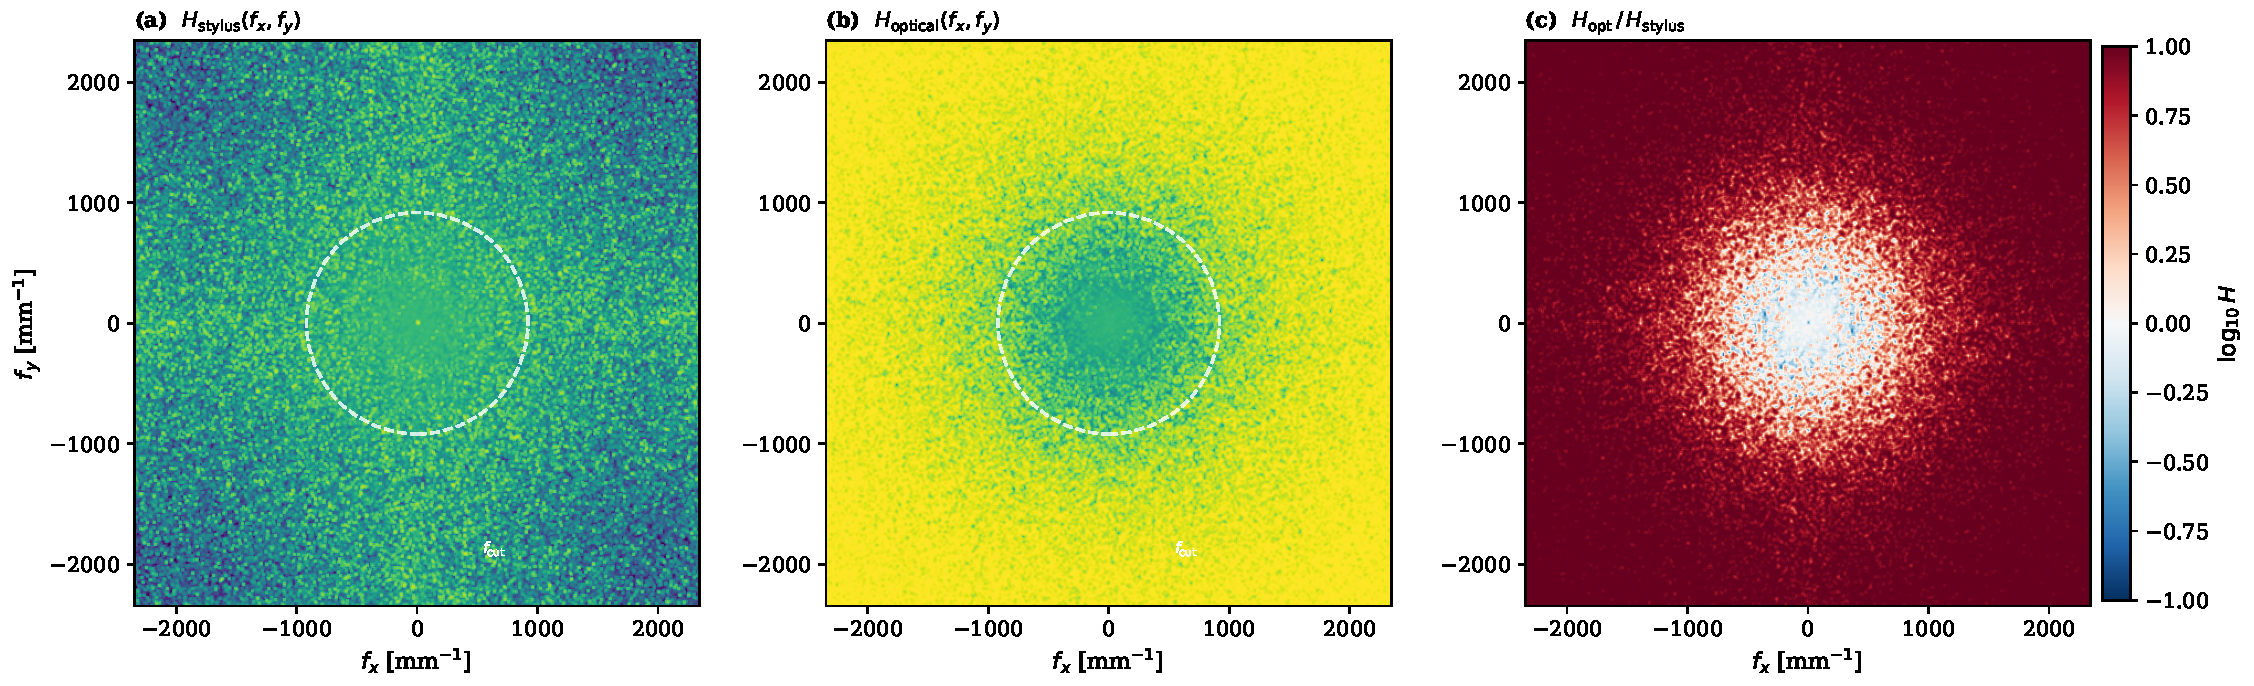
\includegraphics[width=0.48\textwidth]{../../pipeline/outputs/iter01/figures/fig2_transfer_functions}
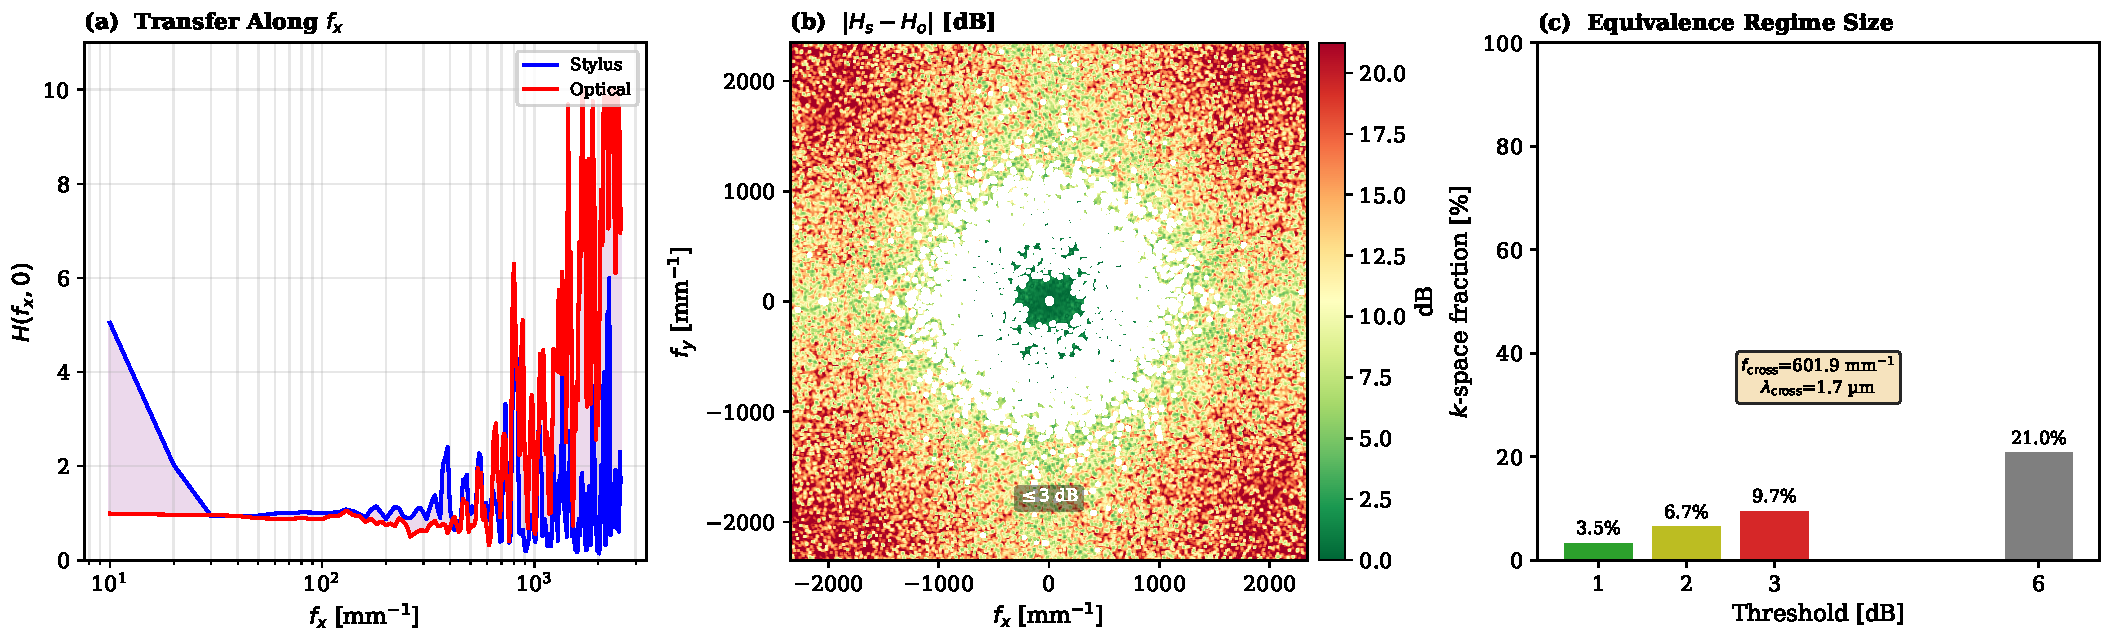
\includegraphics[width=0.48\textwidth]{../../pipeline/outputs/iter01/figures/fig6_crossover_analysis}
\caption{Left: simulated instrument transfer functions in $k$-space --- stylus (flat with curvature-bias excess), optical (diffraction-limited), and their ratio. Right: crossover analysis --- the \qty{3}{\decibel} equivalence boundary and the equivalence fraction as a function of threshold.}
\label{fig:transfer}
\end{figure*}

\textbf{Equivalence regime.} The modalities agree to within \qty{3}{\decibel} over \qty{9.6}{\percent} $\pm$ \qty{0.3}{\percent} of the measured $k$-space ($n=30$ ensemble, $N=512$ grid), with a crossover frequency $f_\mathrm{cross} = \qty{454}{\per\milli\metre} \pm \qty{165}{\per\milli\metre}$ (feature wavelength $\approx$ \qty{2.2}{\micro\metre}). Below the crossover the stylus dominates; above it the optical system retains information up to its diffraction cutoff. A 180-point parameter sweep shows the crossover depends only weakly on the tip radius ($f_\mathrm{cross} \propto r_\mathrm{tip}^{-0.06\pm0.01}$).

\textbf{Accuracy and scaling.} The stylus achieves an rms error of \qty{16.3}{\nano\metre} against the optical \qty{29.3}{\nano\metre}, despite the optical system's higher nominal cutoff: unwrapping errors, not bandwidth, limit the optical accuracy. The sweep is approximately described by an empirical power law $\mathrm{RMSE}_s/\mathrm{RMSE}_o \propto (f_{c,\mathrm{opt}}/f_{c,\mathrm{stylus}})^{1.90\pm0.13}$ (in-sample $R^2 = 0.53$; blocked cross-validation $R^2 = 0.52$), which is reported as an order-of-magnitude descriptor rather than a precise predictor.

\subsection{Information-Theoretic Diagnostics}
\label{sec:diagnostics}
Treating the profilometer as a Gaussian channel \cite{shannon1948mathematical,cover2006elements}---the surface a stationary Gaussian field and the measurement a filtered observation with additive noise---the mutual information between surface and measurement decomposes per spatial frequency,
\begin{equation}
I(h;y) = \frac{1}{2}\sum_{\mathbf{f}}\log_2\!\left[1 + \frac{|H(\mathbf{f})|^2\, S_h(\mathbf{f})}{S_\eta(\mathbf{f})}\right],
\end{equation}
and the minimum mean-square reconstruction error takes the closed form $\mathrm{MMSE} = \sigma^2 - \iint |H|^2 S_h^2/(|H|^2 S_h + S_\eta)\,d^2f$, verified against Monte Carlo Wiener filtering in the verification suite. The reconstructability index $\rho = 1 - \mathrm{MMSE}/\sigma^2$ then favours the stylus at the baseline ($\rho_\mathrm{stylus} = 0.79$ versus $\rho_\mathrm{optical} = 0.64$), and the per-band information loss is lowest at low frequencies (0.071 decades) and highest near the sampling scale (0.446 decades). The total mutual-information ranking is estimator-dependent (ratios of 0.7--1.6 across defensible noise-floor estimators) and is therefore not claimed as robust; only the per-band picture is reported as an estimator-independent result.

\textbf{Surface-class stress test and third modality.} Six surface classes (Gaussian self-affine, anisotropic ground, turned, laser-textured, periodic grating, and biological-like; $n=5$ realisations per class) were analysed to check whether the metrics generalise beyond the calibration class. The reconstructability index is stable across the random rough classes (CV = 0.16) and saturates at unity for strongly deterministic surfaces, where it becomes surface-limited rather than instrument-limited; the optical system's near-zero $\rho$ on the pure periodic grating is correctly explained by the concentration of spectral power at a single $k$-space point. Extending the framework to scatterometry via the Rayleigh--Rice BSDF-to-PSD relation adds a third, flat-response channel spanning \qtyrange{10}{3760}{mm^{-1}} and confirms the complementarity of the three modalities; the multi-instrument fusion of the three estimates is retained as a conceptual outlook (see Section~\ref{sec:applications}). The measurement anisotropy is small for both modalities ($\alpha_s = 0.0095 \pm 0.0038$ versus $\alpha_o = 0.0013 \pm 0.0006$, i.e.\ the stylus exceeds the optical value by a factor of about seven), and the spectral information loss increases mildly with frequency (local log--log slope $\approx 0.4$ over \qtyrange{50}{1500}{mm^{-1}}).

\textbf{Public-data cross-checks.} The optical channel model was benchmarked against the public, CC-BY-4.0 WLI dataset of Hirose et al. \cite{hirose2025topography} (Zenodo 10.5281/zenodo.15750880): fitting only a background PSD amplitude, its slope, and one instrument parameter (the cutoff scale $c$) reproduces the measured instrument transfer functions with $c = 1.15 \pm 0.01$ (Fig.~\ref{fig:benchmark}). The stylus channel admits no comparable paired dataset; as a geometric cross-check, the dilation simulator reproduces the classical parallel-curve radius shift on the published ball-standard calibration profiles of Aksulu \cite{aksulu2021stylus} within \qtyrange{3}{5}{\percent} for tip radii of \qtyrange{2}{50}{\micro\metre}, although the published profiles' scatter (\qtyrange{40}{120}{\micro\metre}) exceeds the tip scale, so this check is geometric rather than tip-resolving.

\begin{table*}[t]
\centering
\caption{Key verified quantities of the study (all from the committed simulation pipeline and its verification suite).}
\label{tab:key}
\begin{tabular}{lll}
\toprule
Quantity & Stylus & Optical \\
\midrule
Transfer at 292 mm$^{-1}$ (empirical power) & 0.91 & follows incoherent OTF \\
$\qty{3}{\decibel}$ point & $\approx$ \qty{1049}{mm^{-1}} & \qty{2000}{mm^{-1}} (cutoff) \\
Baseline rms error & \qty{16.3}{\nano\metre} & \qty{29.3}{\nano\metre} \\
Anisotropy $\alpha$ ($n=30$) & $0.0095 \pm 0.0038$ & $0.0013 \pm 0.0006$ \\
Reconstructability $\rho$ (baseline) & 0.79 & 0.64 \\
\bottomrule
\end{tabular}
\end{table*}

\begin{figure*}[b]
\centering
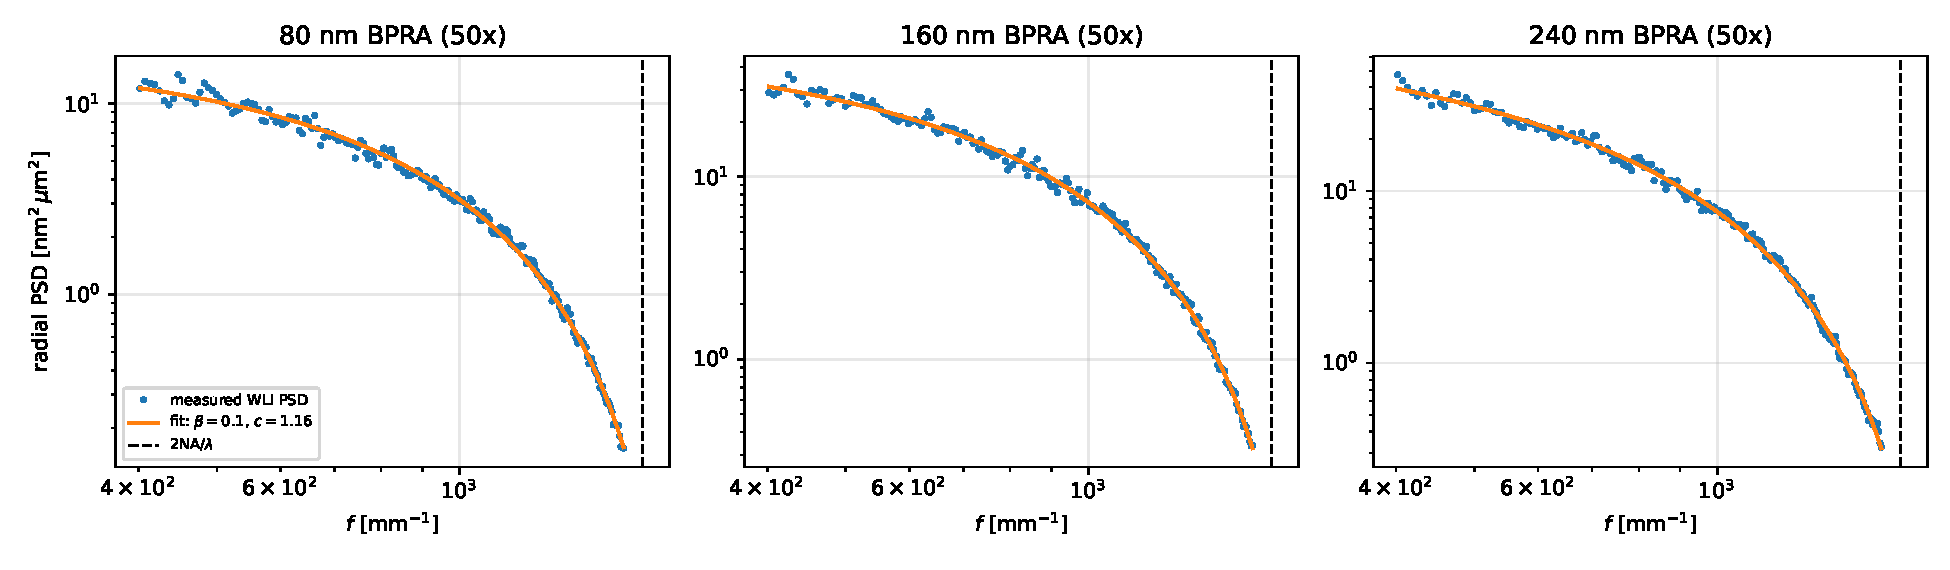
\includegraphics[width=0.95\textwidth]{../../pipeline/outputs/iter01/figures/fig_public_benchmark}
\caption{Public-data validation of the optical channel model: measured WLI radial PSDs (points) of three binary-pseudo-random-array samples (Hirose et al., CC-BY-4.0) and the fitted model (lines) with fitted cutoff scale $c$; the vertical line marks the nominal monochromatic cutoff $2\mathrm{NA}/\lambda$.}
\label{fig:benchmark}
\end{figure*}

\textbf{Gap-closure roadmap.} Because the optical OTF is inherently low-pass while the stylus transfer is nearly flat across most of its passband, optical profilometry cannot fully dominate the stylus in $k$-space, but near-total equivalence is attainable. A 432-point sweep ($N=256$ grid; its own baseline is \qty{48}{\percent}) shows that a $100\times$ noise-floor reduction, NA of 0.7--0.9, shorter illumination wavelengths, and two-dimensional phase unwrapping expand the equivalence fraction from the ensemble baseline of \qty{9.6}{\percent} to \qty{87}{\percent} within the sweep. A bias-limited residual gap remains at the lowest spatial frequencies, where the stylus curvature-bias excess ($+\qty{3.4}{\decibel}$) exceeds the \qty{3}{\decibel} criterion and the stylus remains the primary standard.

\section{Potential Applications}

\label{sec:applications}
The framework gives practitioners quantitative criteria for instrument selection. For feature wavelengths between \qtyrange{0.5}{1.5}{\micro\metre} (frequencies \qtyrange{670}{2000}{mm^{-1}}), the optical measurement is preferred; in the crossover band (\qtyrange{1.5}{2}{\micro\metre}) the two measurements carry comparable information and can be averaged; for wavelengths above \qty{2}{\micro\metre} the stylus is preferred. Below \qty{0.5}{\micro\metre} --- beyond the optical diffraction cutoff --- neither modality resolves surface features in the modelled passband. The crossover frequency serves as a trust boundary for cross-validation of real measurements. The gap-closure roadmap prescribes four instrument improvements with the highest equivalence gain for optical systems: (i) a $100\times$ reduction of the optical noise floor (cooled sCMOS detectors, brighter illumination and multi-frame averaging); (ii) higher numerical apertures (0.7--0.9); (iii) shorter illumination wavelengths (\qtyrange{400}{450}{\nano\metre}); and (iv) two-dimensional quality-guided phase unwrapping in place of one-dimensional row unwrapping. For instrument qualification, the transfer-function framework complements scalar benchmarks: two instruments with equal rms error can differ markedly in the spatial-frequency bands they preserve, and the equivalence boundary provides a quantitative cross-validation rule. A $k$-space fusion of stylus, WLI and scatterometry, weighted by local information uncertainty, is presented as a conceptual outlook rather than a quantitative validation, since the simulated scatterometry PSD is not yet on the same absolute scale as the height PSD.

\section{Conclusions}

\label{sec:conclusions}
A paired, first-principles $k$-space comparison of stylus and optical profilometry was developed and verified. Its central, reproducible findings are: (i) the stylus transfer is approximately flat with a curvature-bias excess and rolls off only near the sampling scale, in contrast to the classical Gaussian-tip picture, which underestimates the transfer by two orders of magnitude; (ii) the optical transfer follows the incoherent OTF and reproduces measured public WLI transfer functions; (iii) the modalities are interchangeable over \qty{9.6}{\percent} $\pm$ \qty{0.3}{\percent} of $k$-space with a quantitative crossover at $\approx$ \qty{454}{mm^{-1}}; and (iv) the gap between the modalities can be narrowed to \qty{87}{\percent} equivalence with four prescribed instrument improvements. All results are computational and are offered with a falsifiable experimental roadmap; an experimental realisation with calibrated artefacts remains the decisive next step. The complete simulation framework, including the eighteen-test verification suite and the audit scripts behind every reported number, is available in a public repository~\cite{kucharski2026repository} (release v1.0.2, Zenodo DOI 10.5281/zenodo.23493875).

\section*{AUTHORS' CONTRIBUTION}

Dawid Kucharski: conceptualisation, methodology, software, formal analysis, investigation, validation, writing --- original draft, writing --- review and editing. Micha{\l} Jakubowicz: visualisation.

\bibliographystyle{imeko_wc}
\bibliography{imeko-wc-abstract}

\end{document}
